\chapter{Data Stratification}
\label{chapter:data_stratification}

To gain a deeper understanding of the properties of the data in the \ac{iemo} dataset, we conducted data stratification. Our objective was to group the classification labels based on several attributes of the dataset, explore their properties, and potentially identify any limitations these properties may impose on machine learning models in the \ac{ser} field.

\section{Recordings Durations}

The duration of an audio recording can significantly impact the analysis and modeling of the data. We hypothesize that shorter recordings may not capture enough information to adequately represent the signal of interest, while longer recordings may contain irrelevant or redundant information. For this matter, we stratified the dataset based on the duration of the recordings.

The dataset contains recordings ranging from approximately 0.25 to 34 seconds in duration, and we divided the recordings into three evenly balanced groups, in terms of the number of recordings: short, less than or equal to  2.29 seconds, medium, greater than 2.29 and less than or equal to 4.38 seconds, and long, greater than 4.38 seconds.

Table \ref{5:durations} presents the impact of the duration of the recordings on the performance of the chosen traditional \ac{xgb} model. The longest recordings have the highest performance, with an accuracy of 63.77\%.

\begin{table}[H]
	\centering
	\caption{Traditional model 5-fold cross-validation results on stratitifed data based on the recordings' duration.}
	\label{5:durations}
	\begin{tabular}{lrlrrrr}
		\toprule
		Recordings Duration &   Total Data & Accuracy    &   Macro F1 &   Precision &   Recall &   \ac{mcc} \\
		\midrule
		Short ($]0, 2.29]$ s)	 	&      1844 & 55.69$\pm$1.15 &   54.64 &  56.59 &  53.54 &  0.38  \\
		Medium ($]2.29, 4.38]$ s) 	&      1843 & 56.65$\pm$2.28 &   57.16 &  57.25 &  57.26 &  0.41 \\
		Long ($]4.38, 34]$ s) 		&      1844 & 63.77$\pm$0.87 &   64.16 &  64.32 &  64.17 &  0.51  \\	
		\bottomrule
	\end{tabular}
\end{table}

The obtained classification results suggest that longer recordings are easier for the model to classify accurately, as they provide more information. This allows us to conclude that recordings' duration has a substantial performance impact on the \ac{ser} task and is a significant factor to consider when building classification models.

\section{Speaker Gender}

Another attribute we used for stratification was the gender of the speaker. The dataset contains a similar amount of recordings from speakers of both genders, having 2649 recordings with female speakers and 2882 with male speakers.

To evaluate the classification performance on different genders, we trained and tested the model on recordings from female speakers, male speakers, and mixed-gender recordings. Table \ref{5:gender} shows the 5-fold cross-validation results of the traditional model on each category.

\begin{table}[H]
	\centering
	\caption{Traditional model 5-fold cross-validation results on stratitifed data based on speaker gender recordings.}
	\label{5:gender}
	\begin{tabular}{llrrrrr}
		\toprule
		Training Gender & Testing Gender & Accuracy    &   Macro F1 &   Precision &   Recall &   \ac{mcc} \\
		\midrule
		Female 	& Female & 59.95$\pm$1.45 & 60.47 &       60.4  &    60.77 &   0.46 \\
		Male 	& Male   & 59.99$\pm$1.28 & 60.67 &       61.38 &    60.2  &   0.45 \\
		
		\addlinespace

		Female  & Male	 & 50.28$\pm$0.64 &  50.57 &       50.36 &    51.1  &   0.32 \\
		Male    & Female & 49.41$\pm$1.43 &  50.26 &       53.37 &    49.24 &   0.32 \\
		\bottomrule
	\end{tabular}
\end{table}

From the table, it can be observed that the model performed similarly on both genders, when the testing data's gender is equal of the training data's gender, with accuracies close to 60\%. However, when testing on the opposite gender of the training, the model's accuracy dropped significantly to 50.28\% and 49.41\% for female and male trained models, respectively. The other metrics showed equivalent behavior, indicating difficulty in correctly identifying the emotion in mixed-gender contexts.

These results suggest that the model's performance is affected by the gender of the speakers in the training data and therefore, it is important that the model is provided with a gender-balanced set of training data to reduce gender bias.

\section{Discrete Emotions}

This section examines the classification performance of different emotional categories in the \ac{iemo} dataset. The dataset contains four emotional categories: anger, happiness, sadness, and neutral. We performed data stratification based on these labels, as well as grouping them based on emotional planes, resulting in 15 groups of data. Table \ref{tab:emo_cat} displays the traditional model's 5-fold cross-validation results on stratitifed data based on discrete emotions. The last two rows of the three and two label cases combine the labels based on their distribution in the arousal and valence planes, respectively.

In the three label case, the best performance was achieved when classifying between anger (high arousal and dominance), neutral, and sadness (low arousal and dominance), with an accuracy and macro F1 score of 75\%. The lowest results were obtained with emotions far apart in the valence plane, such as anger or sadness (low valence), neutral, and happiness (high valence). The last two rows of the three-label case support the same conclusion.

In the two-label case, where the emotional categories were paired, the best performance was achieved when classifying between angry and sad, with an accuracy and macro F1 score of 92\%. However, this group had the least amount of total data. The worst performance was achieved when classifying between neutral and happy, with an accuracy and macro F1 score of around 73\%, which had more total data to classify. Similar to the three-label case, the model achieved better results when classifying labels far apart on the arousal or dominance planes, and worse in the valence plane.

\begin{table}[H]
	\centering
	\caption{Traditional model 5-fold cross-validation results on stratitifed data based on the discrete emotions.}
	\label{tab:emo_cat}
	\resizebox{\textwidth}{!}{%
	\begin{tabular}{lrrrrrr}
		\toprule
		Labels                      &   Total Data & Accuracy    & Macro F1    & Precision   & Recall      & \ac{mcc}       \\
		
		\toprulec
		\rowcolor{gray!25}
		\multicolumn{7}{c}{Four Labels} \\
		\midrulec
		
		Angry, Happy, Sad, Neutral             &         5531 &  60.69$\pm$1.37	& 61.32	& 61.66	& 61.19	& 0.47 \\
		
		\toprulec
		\rowcolor{gray!25}
		\multicolumn{7}{c}{Three Labels} \\
		\midrulec
		
		Angry, Neutral, Sad                 &         3895 & 75.17$\pm$0.99	&	75.30	& 76.21	& 74.62	& 0.62 \\
		Angry, Happy, Sad                   &         3823 & 70.99$\pm$1.55		&71.37	& 71.38	& 71.42	& 0.56 \\
		Sad, Neutral, Happy                 &         4428 & 65.74$\pm$1.85	&	65.85	& 65.94	& 65.86	& 0.48 \\
		Angry, Neutral, Happy               &         4447 & 64.29$\pm$1.13		&63.81	& 64.41	& 63.60	& 0.45 \\
		
		\addlinespace[2mm]
		
		Sad, Neutral, Happy+Angry &         5531 & 69.32$\pm$1.24 &      67.29 &       67.44 &    67.2  &   0.50  \\
		Angry+Sad, Neutral, Happy &         5531 & 60.64$\pm$1.36 &      59.72 &       60.03 &    59.73 &   0.40  \\
		
		\toprulec
		\rowcolor{gray!25}
		\multicolumn{7}{c}{Two Labels} \\
		\midrulec
		
		Sad, Angry                          &         2187 & 92.00$\pm$1.30 & 	92.00	&  92.00 & 	92.00 & 	0.84 \\
		Angry, Neutral                      &         2811 & 84.53$\pm$1.26 &	83.49& 	84.25& 	82.98& 	0.67 \\
		Sad, Happy                          &         2720 & 83.79$\pm$0.85 &      83.10  &       83.08 &    83.11 &   0.66 \\
		Sad, Neutral                        &         2792 & 81.02$\pm$1.16 &      79.70  &       80.29 &    79.29 &   0.60  \\
		Angry, Happy                    	&         2739 & 75.58$\pm$0.93 &      74.15 &       74.78 &    73.79 &   0.49 \\
		Happy, Neutral                      &         3344 & 73.24$\pm$1.06 &      73.15 &       73.34 &    73.15 &   0.46 \\
		
		\addlinespace[2mm]
		
		Sad+Neutral, Happy+Angry  &         5531 & 77.24$\pm$1.04 & 77.21 & 77.31 &	77.21 & 0.55 \\
		Angry+Sad, Neutral+Happy  &         5531 & 73.82$\pm$0.77 &	71.70 & 72.90 & 71.21 & 0.44 \\

		\bottomrule
	\end{tabular}%
	}
\end{table}


It is worth noting that the total data impacts the classification, as a lower number of files may make the classification easier. However, the results suggest that a classification model is better at distinguishing emotional categories that are distant in the arousal or dominance planes than in the valence plane. For instance, anger and happiness (high arousal and dominance) are easier for a model to distinguish between sadness (lower arousal and dominance), while the model has a harder time classifying anger and sadness (low valence) between happiness (high valence).

Based on our analysis, we suggest that the subjectivity of emotions, along with the distribution on emotional planes, may contribute to the difficulty in accurately classifying certain emotional categories, especially happiness and neutral. Hence, it is imperative to develop emotional datasets with a high degree of confidence, utilizing robust labeling techniques that consider the distribution of emotions across different emotional planes. This approach can help enhance the performance of machine learning models in the field of \ac{ser}.


\section{Dimensional Emotions}

In addition to the categorical classification, we also explored the dimensional annotations of the dataset in terms of valence (ranging from unpleasant to pleasant), arousal (ranging from calm to excited), and dominance (ranging from submissive to dominant). These dimensions were rated on a continuous scale of 1 to 5 by human judges.

Initially, we aimed to investigate the level of difficulty associated with classifying each emotional dimension, so we utilized traditional approach features to assess the performance of a \ac{rf} Regressor model from sklearn for each dimension. Each dimension underwent 5-fold cross-validation. We used \ac{mae}, \ac{rmse}, and $R^2$ as evaluation metrics for the model.

Table \ref{tab:dim_reg} shows the results of our experiments on the regression task. The arousal and dominance dimensions are easier to classify than valence. One possible reason for this is that valence is a more complex and abstract concept that may be more difficult to recognize and classify in speech. Additionally, the annotations for valence may be more subjective and varied among annotators than the others, leading to less reliable labels and lower classification performance.


\begin{table}[H]
	\centering
	\caption{\ac{rf} Regressor 5-fold cross-validation using dimensional emotions as labels.}
	\label{tab:dim_reg}
	\begin{tabular}{lrrr}
		\toprule
		Regression Labels   &   \ac{mae} &  \ac{rmse} & $R^2$ \\
		\midrule
		Valence             & 0.700 & 0.859 & 0.182 \\
		Arousal             & 0.414 & 0.522 & 0.520 \\
		Dominance           & 0.534 & 0.657 & 0.362 \\
		\bottomrule
	\end{tabular}
\end{table}

We conducted a comparison between the discrete and dimensional annotations by calculating the means of each dimensional label based on the discrete one. These means, known as dimensional centroids, are presented in Table \ref{tab:dis_dim} and in a 2D plane \ref{fig:2dplane}. To determine if the centroids are accurate or too distant from the expected values, we compared them with the state-of-the-art Russell and Mehrabian's \ac{vad} model.

\begin{table}[H]
	\centering
	\caption{\ac{iemo} dimensional centroids and comparison to the \ac{vad} model.}
	\label{tab:dis_dim}
	\begin{tabular}{lrrr}
		\toprule
		\multirow{2}{*}{\begin{tabular}[c]{@{}l@{}}Emotion\end{tabular}}  & \multicolumn{3}{c}{Centroids} \\ \cmidrule{2-4}
		&  Arousal &   Valence & Dominance \\
		\midrule
		VAD Anger     & 4.34 & 2.14 & 3.68 \\
		VAD Happiness & 3.96 & 4.52 & 3.70 \\
		VAD Neutral   & 3.00 & 3.00 & 3.00 \\
		VAD Sadness   & 3.54 & 1.74 & 2.34 \\
		\addlinespace
		Anger   	&   3.64 \textcolor{red}{$(-0.70)$} &  1.91 \textcolor{red}{$(-0.23)$} &  3.95 \textcolor{green}{$(+0.27)$} \\
		Happiness   &   3.41 \textcolor{red}{$(-0.55)$} &  3.95 \textcolor{red}{$(-0.57)$} &  3.23 \textcolor{red}{$(-0.47)$} \\
		Neutral 	&   2.73 \textcolor{red}{$(-0.27)$} &  2.97 \textcolor{red}{$(-0.03)$} &  2.83 \textcolor{red}{$(-0.17)$} \\
		Sadness     &   2.56 \textcolor{red}{$(-0.98)$} &  2.25 \textcolor{green}{$(+0.51)$} &  2.83 \textcolor{green}{$(+0.49)$} \\
		\bottomrule
	\end{tabular}
\end{table}


\begin{figure}[H]
	\centering
	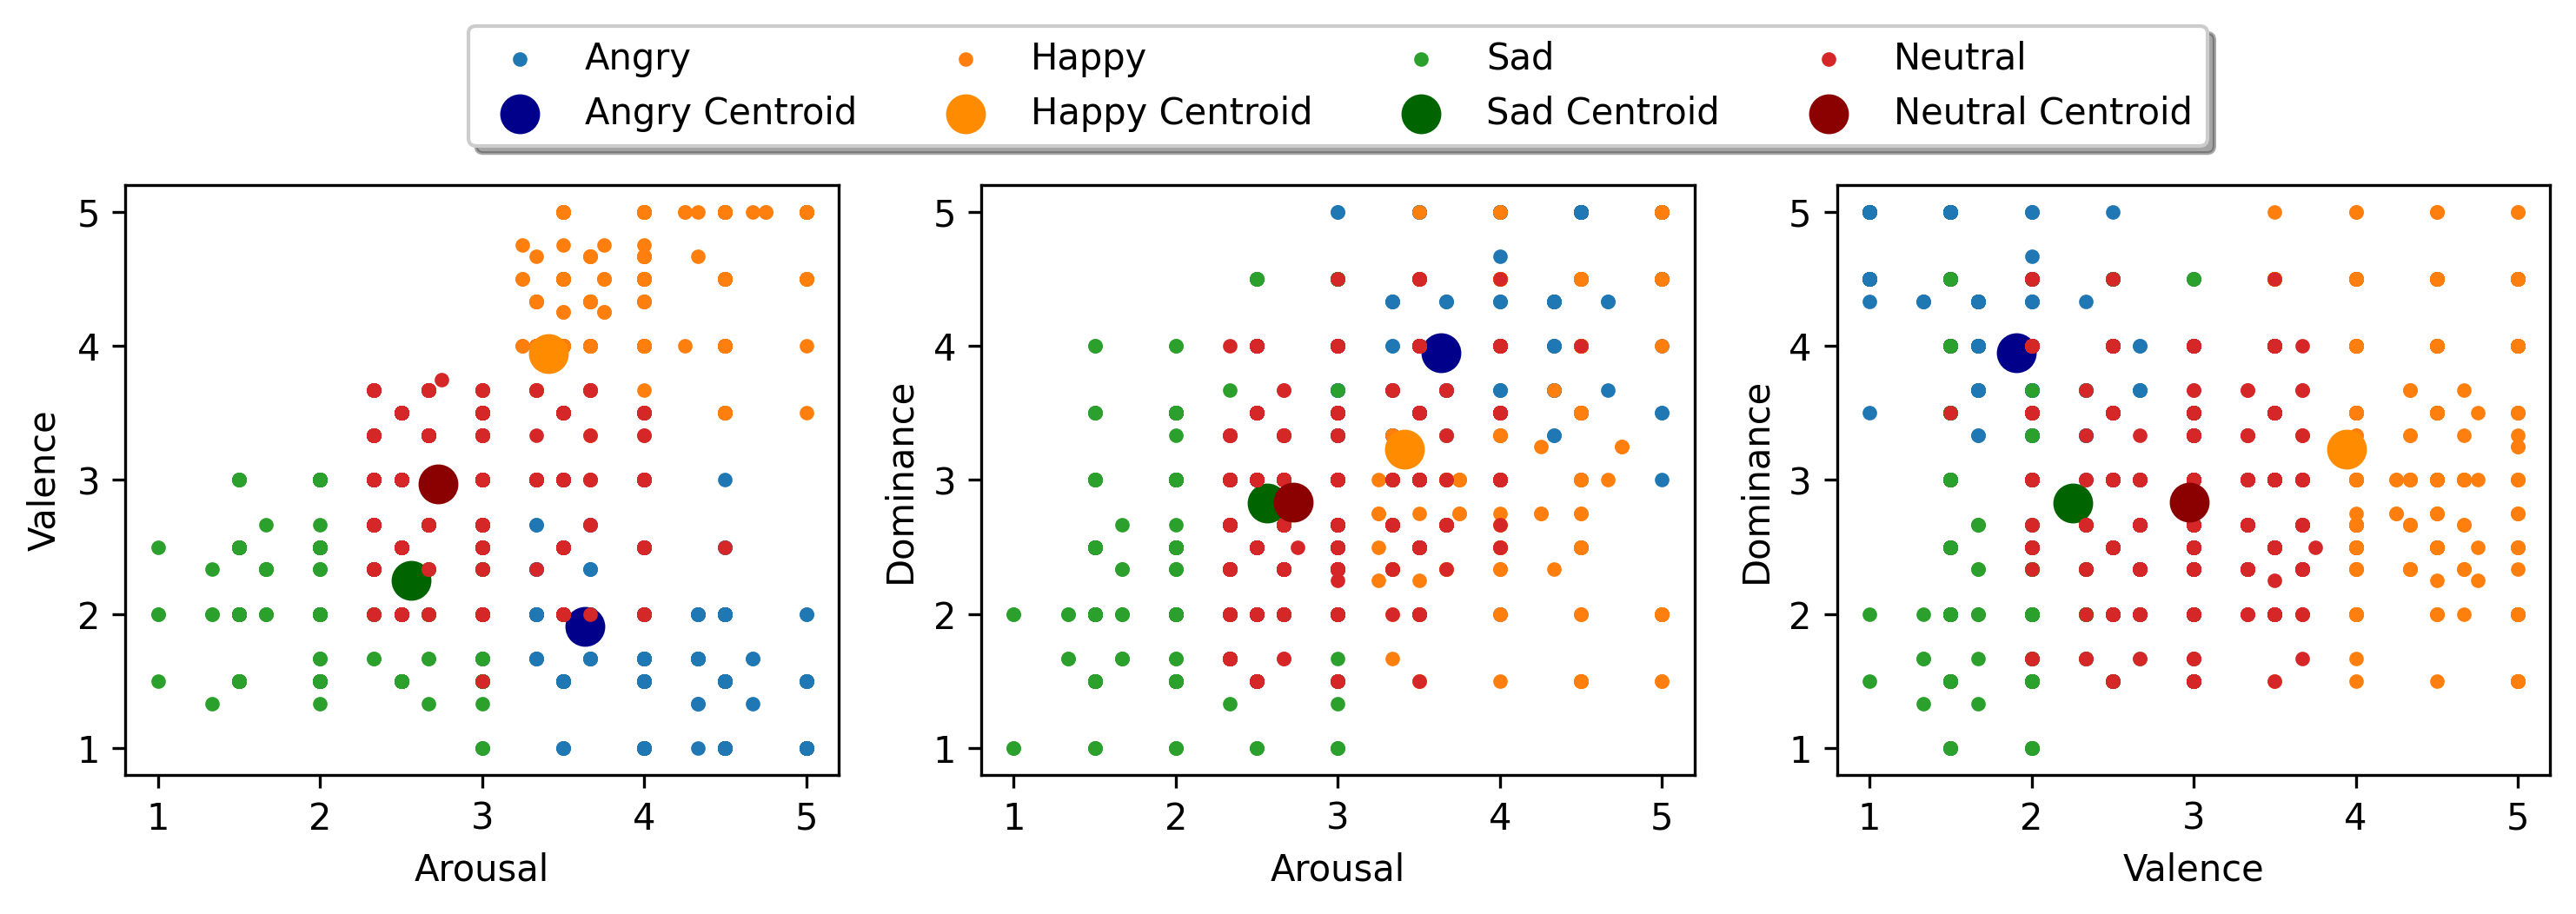
\includegraphics[width=.9\linewidth]{figs/5_data_stratification/primitives_visualization_2d.png}
	\caption{2D representation of the \ac{iemo} and \ac{vad} model dimensional centroids.}
	\label{fig:2dplane}
\end{figure}

The results indicate that the centroids of each discrete emotion have some differences to the \ac{vad} model. For the arousal dimension, it was noted that all emotions have lower values, with sadness showing a greater deviation. In terms of valence, the annotations are more comparable to the \ac{vad} model, but sadness contradicts the lower trend of the other two emotions. The annotations on the dominance dimension also vary the deviation trends.

Based on this, we decided to remove any data that contains dimensional annotations far from the \ac{vad} model centroids for each discrete emotion. Table \ref{tab:conf} demonstrates this conflicts removal process between each emotion's categories and the respective dimensional annotations.

\begin{table}[H]
	\caption{Maintained dimensional annotations range for each emotion category.}
	\label{tab:conf}
	\centering
	\begin{tabular}{lrrr}
		\toprule
		\multirow{2}{*}{\begin{tabular}[c]{@{}l@{}}Emotion\end{tabular}} & \multicolumn{3}{c}{Ranges Maintained} \\ \cmidrule{2-4}
		&    Arousal &      Valence &       Dominance \\
		\midrule
		Angry   &   $]2, 5]$  	& $[1, 4.5]$ 	&  None 		\\
		Happy 	&   $[2.5, 5]$  & $[3, 5[$ 		&  None 		\\
		Sad    	&   $]2, 5]$ 	& $[1, 4]$ 		&  $[1, 4]$ 	\\
		Neutral &   $]2, 4[$	& $[2, 4]$ 		&  $]2, 4[$		\\
		\bottomrule
	\end{tabular}
\end{table}

With this process, 1136 audio files were removed, and 4395 audio files were retained. The new \ac{vad} centroids calculated, as shown in table \ref{tab:new_c}, were closer to the numeric values of the \ac{vad} emotion centroids. Figure \ref{fig:2dplane2} depicts a 2D visualization of the centroids of the \ac{vad} model, along with the data with and without dimensional conflicts. The visualization indicates that the centroids are now closer to the \ac{vad} emotion centroids after the conflicts removal process, which is a possible indication that the conflict-free data is more suitable for the \ac{ser} task.

\begin{table}[H]
	\centering
	\caption{\ac{iemo} dimensional centroids and comparison to the \ac{vad} model after the conflicts removal process.}
	\label{tab:new_c}
	\begin{tabular}{lrrr}
		\toprule
		\multirow{2}{*}{\begin{tabular}[c]{@{}l@{}}Emotion\end{tabular}} & \multicolumn{3}{c}{Centroids} \\ \cmidrule{2-4}
		&  Arousal  &   Valence  & Dominance \\
		\midrule
		Anger   	&   3.78 \textcolor{red}{$(-0.56)$} &  1.86 \textcolor{red}{$(-0.28)$} &  4.02 \textcolor{green}{$(+0.34)$} \\
		Happiness   &   3.49 \textcolor{red}{$(-0.47)$} &  4.00 \textcolor{red}{$(-0.52)$} &  3.39 \textcolor{red}{$(-0.31)$} \\
		Neutral 	&   2.75 \textcolor{red}{$(-0.25)$} &  3.03 \textcolor{red}{$(-0.03)$} &  2.96 \textcolor{red}{$(-0.04)$} \\
		Sadness     &   2.47 \textcolor{red}{$(-1.07)$} &  2.05 \textcolor{green}{$(+0.31)$} &  2.61 \textcolor{green}{$(+0.27)$} \\
		\bottomrule
	\end{tabular}
\end{table}


\begin{figure}[H]
	\centering
	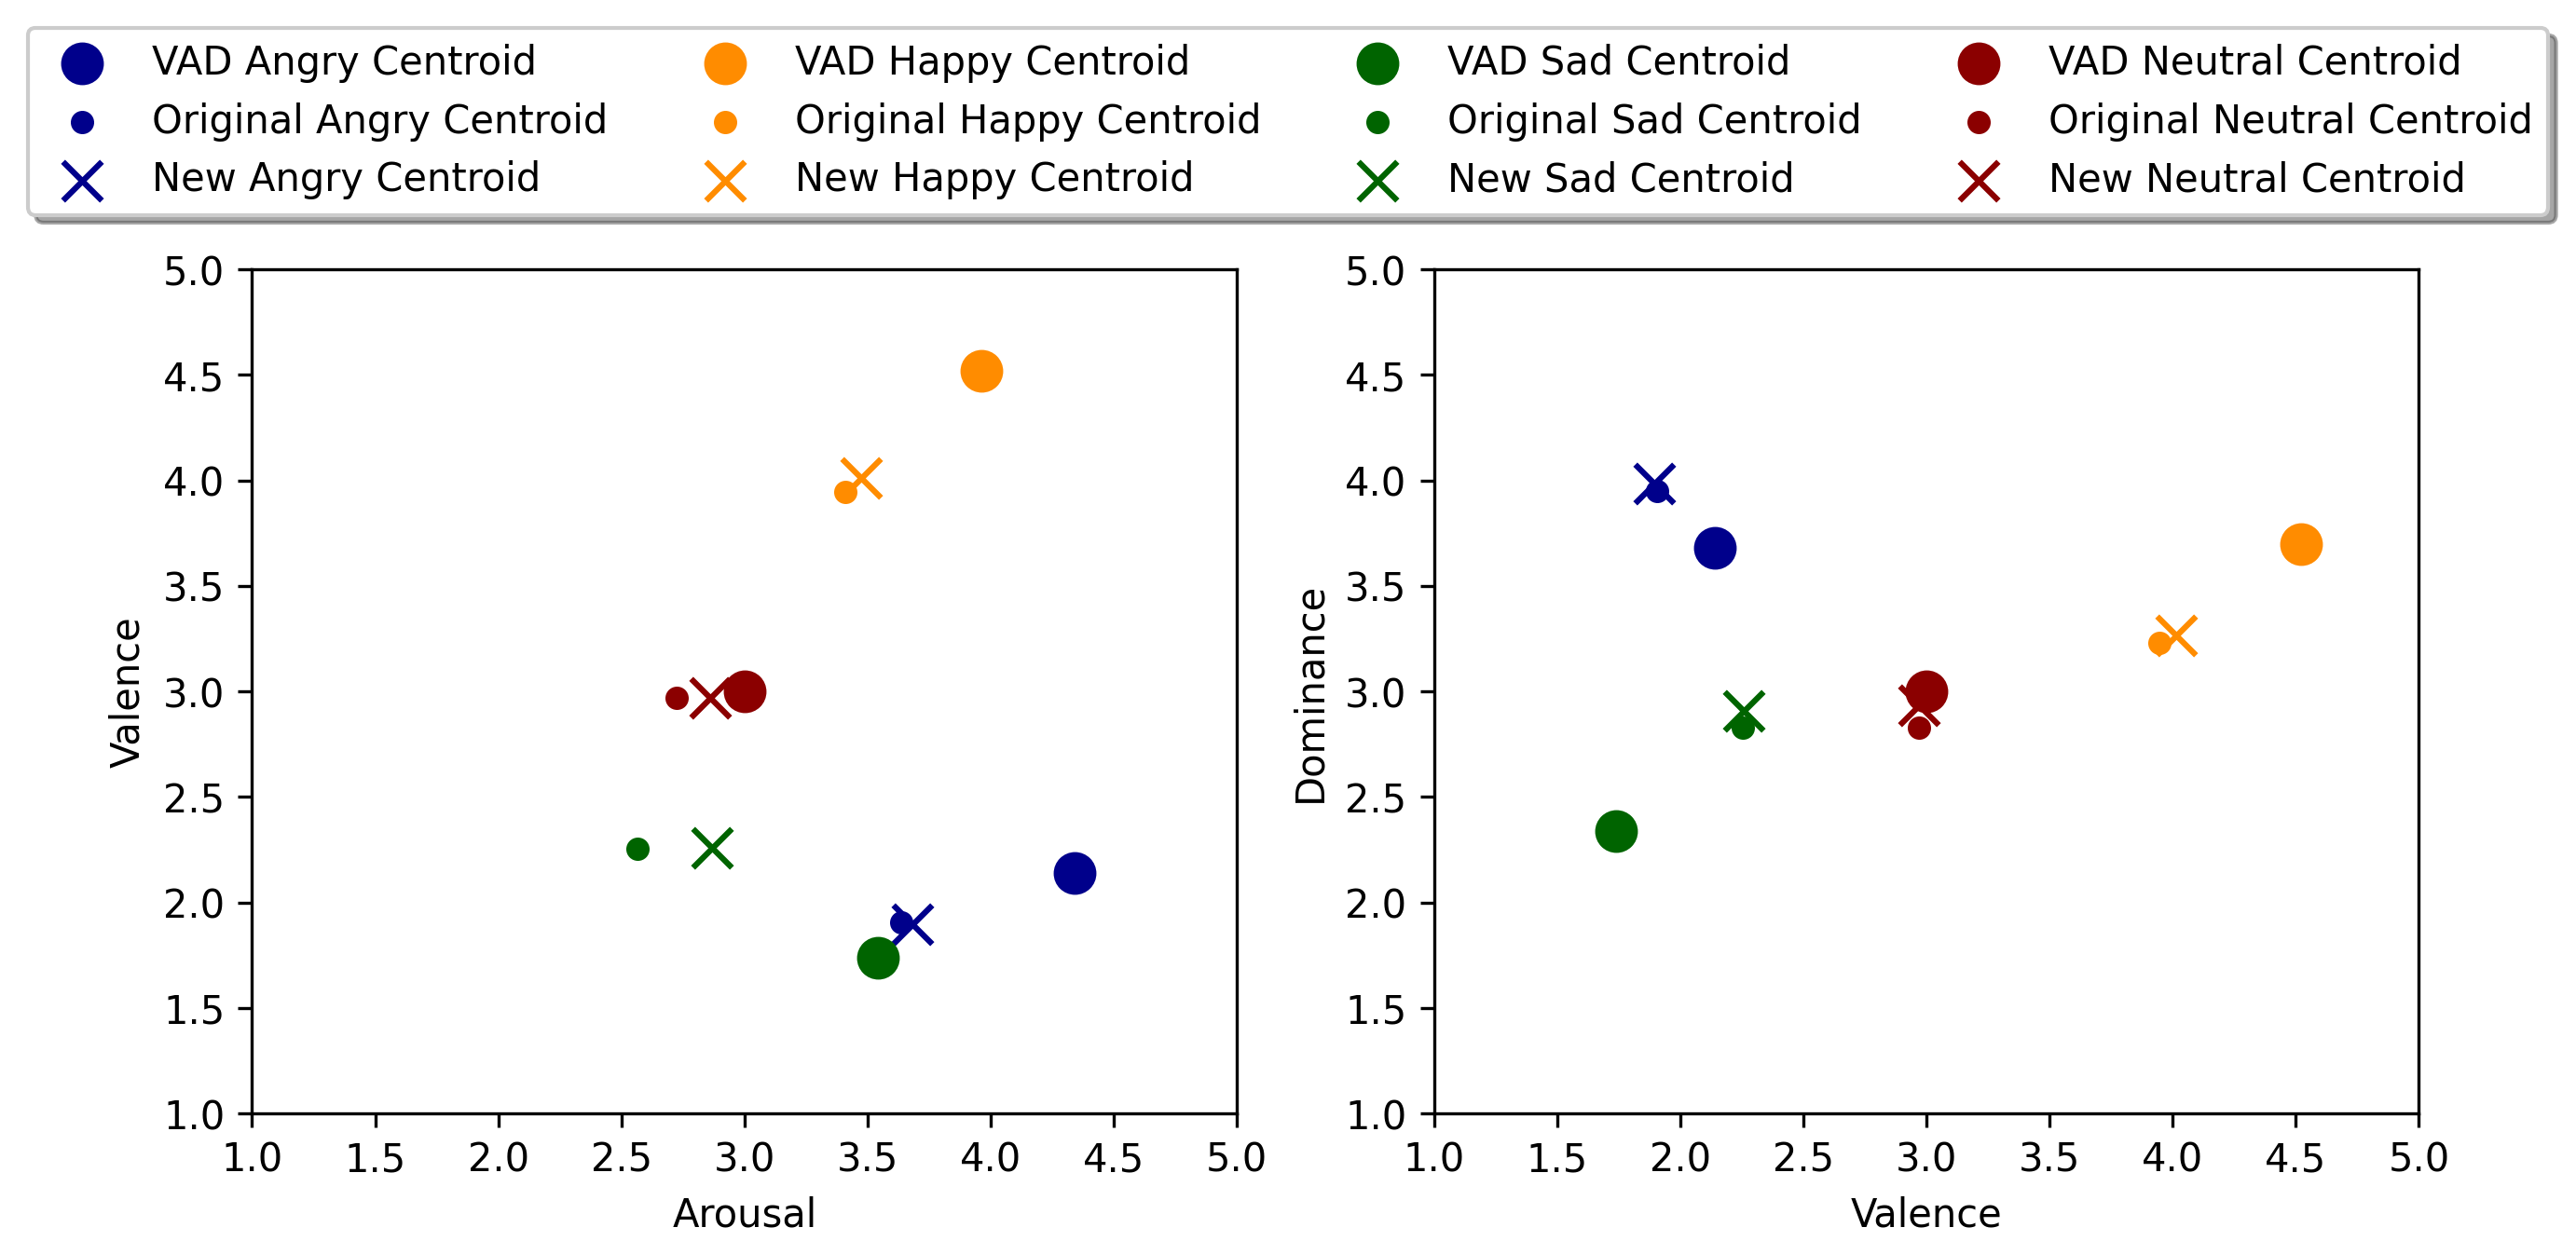
\includegraphics[width=.9\linewidth]{figs/5_data_stratification/strict_conflicts_centroids_2d.png}
	\caption{2D visualization of the entire \ac{iemo} data, along with the conflict-free data and the \ac{vad} model's dimensional centroids.}
	\label{fig:2dplane2}
\end{figure}

To evaluate further if this removal of data translates to cleaner data and, therefore, to a more effective emotion recognition process, a 5-fold cross-validation was performed using that conflict-free data and compared against the results obtained using the complete dataset. The results are shown in Table \ref{tab:emo_cat2}, and they indicate that the conflict-free dataset outperforms the complete dataset in all metrics. While this outcome supports our hypothesis, the observed improvements are not significant enough to attribute them solely to the removal of data based on dimensional annotations. Other random variables, such as variations in emotion distributions across folds or the decrease in the total number of files, could also have contributed to the observed improvements. Hence, further investigation is required to establish the actual impact of this process.

\begin{table}[H]
	\small
	\centering
	\caption{Traditional model 5-fold cross-validation results with the conflicts removal process.}
	\label{tab:emo_cat2}
	\centering
	\begin{tabular}{lrrrrrr}
		\toprule
		Data   & Total Data						 	& Accuracy    & Macro F1    & Precision   & Recall      & \ac{mcc}       \\
		\midrule
		All Data & 5531 & 60.69$\pm$1.37 & 61.32 & 61.66 & 61.19 & 0.470 \\
		Conflict-Free Data & 4456 & 62.01$\pm$1.74 & 63.00 & 63.36 & 62.76 & 0.480 \\
		\bottomrule
	\end{tabular}
\end{table}


\subsection{Conclusion}

The data stratification process enabled us to uncover the shortcomings of the \ac{iemo} dataset and the model we developed. Having obtained valuable insights from our observations and conclusions on the subsections about duration, gender, and dimensional annotations, we aim to utilize the training data in our model to enhance its reliability and performance. In light of this, we have decided to train both traditional and \ac{dl} models on data that aligns with our objectives.

To achieve this, to the conflict-free data obtained from the dimensional conflict removal process, we applied an additional file duration condition. Specifically, we only retained audio files with a duration exceeding 1 second, as it was necessary to ensure the presence of sufficient emotional data for the model to learn effectively. As a result of this process, we obtained a total of 4200 audio files, with a nearly balanced gender distribution, comprising 52.9\% male and 47.1\% female speakers.

Table \ref{tab:emo_cat3} presents the 5-fold cross-validation results of the traditional model trained on the \ac{iemo} dataset with different sets of selected data. The first row shows the results obtained with all 5531 files of the dataset. The second row shows the results after applying the dimensional conflict removal process, resulting in 4395 files. The third row shows the results of the conflict-free data with the previously mentioned additional duration condition, resulting in 4200 audio files. The results demonstrate that the performance of the traditional model improves as the data selection process becomes more rigorous. The dimensional conflict removal process resulted in an increase in accuracy from 60.69\% to 62.01\%, while the additional duration condition further improved the accuracy to 62.89\%, the other metrics exhibit similar improvements, indicating that the model's classification ability improved with the use of cleaner and more reliable data.

\begin{table}[H]
	\small
	\centering
	\caption{Traditional model 5-fold cross-validation results different sets of data.}
	\label{tab:emo_cat3}
	\centering
	\begin{tabular}{lrrrrrr}
		\toprule
		Data   	&	Total Data &	Accuracy    & Macro F1    & Precision   & Recall      & \ac{mcc}       \\
		\midrule
		All		      & 5531 & 60.69$\pm$1.37 & 61.32 & 61.66 & 61.19 & 0.470 \\
		Conflict-Free & 4456 & 62.01$\pm$1.74 & 63.00 & 63.36 & 62.76 & 0.480 \\
		\begin{tabular}[l]{@{}l@{}}Conflict-Free With\\Duration Condition\end{tabular} & 3347 & 62.89$\pm$0.67 & 63.76 & 63.66 & 63.90 & 0.500 \\
		\bottomrule
	\end{tabular}
\end{table}

Removing conflicts from the dataset results in better performance metrics for our models, however, this approach comes reduces the amount of data which may be the reason for these improvements. To verify if the model does improve, we decided to train and save both traditional and \ac{dl} models with the data that met our set of conditions. These saved models are called stratified models. We then repeated the process made in the previous section and evaluated them on three different datasets, namely eNTERFACE'05, CREMA-D, and EMO-DB.

As shown in Table \ref{strat_final_models}, the stratified models outperformed the previous models trained on all of the \ac{iemo} data on most metrics, which demonstrates that our stratification study resulted in an improved cross-dataset performance of the models.

\begin{table}[H]
	\centering
	\caption{Final models trained on \ac{iemo} and evaluated on different datasets.}
	\label{strat_final_models}
	\resizebox{\textwidth}{!}{%
		\rowcolors{2}{gray!25}{white}
		\begin{tabular}{llrrrrr}
			\toprule
			Dataset & Model & Accuracy & Macro F1 & Precision & Recall & \ac{mcc} \\
			\midrule
			\addlinespace[1mm]
			
			eNTERFACE'05 & Traditional & 32.22 & 17.25 & 29.09 & 24.17 & 0.080 \\
			& Stratified Traditional & 32.38 & 16.11 & 29.23 & 24.29 & 0.077 \\
			& \ac{dl} & 36.67 & 22.91 & 44.36 & 27.50 & 0.087 \\
			& Stratified \ac{dl} & 37.14 & 22.39 & 43.51 & 27.86 & 0.073 \\
			
			\midrulec
			\addlinespace[1mm]
			
			EMO-DB & Traditional & 38.35 & 15.82 & 14.80 & 26.06 & 0.065 \\
			& Stratified Traditional & 38.64 & 16.82 & 35.42 & 26.48 & 0.077 \\
			& \ac{dl} & 38.35 & 15.79 & 37.78 & 25.99 & 0.066 \\
			& Stratified \ac{dl} & 38.05 & 15.22 & 34.71 & 25.63 & 0.052 \\
			
			\midrulec
			\addlinespace[1mm]
			
			CREMA-D & Traditional & 45.22 & 38.96 & 47.62 & 46.41 & 0.315 \\
			& Stratified Traditional & 46.06 & 39.90 & 47.85 & 46.79 & 0.313 \\
			& \ac{dl} & 54.14 & 47.71 & 51.68 & 52.98 & 0.407 \\
			& Stratified \ac{dl} & 55.29 & 50.06 & 54.11 & 54.05 & 0.417 \\
			\bottomrulec
		\end{tabular}%
	}
\end{table}

